\section{"Ubersicht verschiedener Barcodesysteme}
Zur Zeit befinden sich viele verschiedene Barcodesysteme in Benutzung. Manche sind spezifisch für einen bestimmten Wirtschaftszweig, andere wiederum findet man so gut wie überall. Dieser Abschnitt soll die bekanntesten und verbreitetsten Systeme vorstellen. Dabei wird eine Grobeinteilung anhand der Anzahl der Dimensionen des Codes vorgenommen.

\subsection{Eindimensionale Barcodes}
Eindimensionale Barcodes codieren Daten entlang ihrer Länge (also links und rechts); nicht ihrer Höhe (also oben und unten). Würde man nun eine Linie durch einen eindimensionalen Barcode ziehen, findet man diese Dimension. Dieses Vorgehen nutzen die meisten der verwendeten Laserscanner. Dass eindimensionale Barcodes meist sehr groß abgedruckt sind hat einen einfachen Grund: Je größer der Code, desto einfacher findet ihn ein Scanner.

\subsubsection{Strichcode}
Für den Strichcode gibt es seit 1993 vier europäische Standards, die sich durch Einsatzgebiet (Handel/Industrie), Zeichenvorrat und Zeichensatz unterscheiden: ISO 15420 (EAN), ISO 15417 (Code 128), ISO 16388 (Code 39) und ISO 16390 (Code 2/5 Interleaved).
Der Strichcode wird vielfältig eingesetzt und heißt je nach Einsatzgebiet auch anders. Im Handel kennt man ihn unter der Bezeichnung EAN (European Article Number), in den Bereichen Materialfluss, Logistik und Lager als EAN128.
\begin{figure}[htbp]%[7]{r}[0.75cm]{0.4\textwidth}
	\centering
	%\vspace{-0.2cm}
	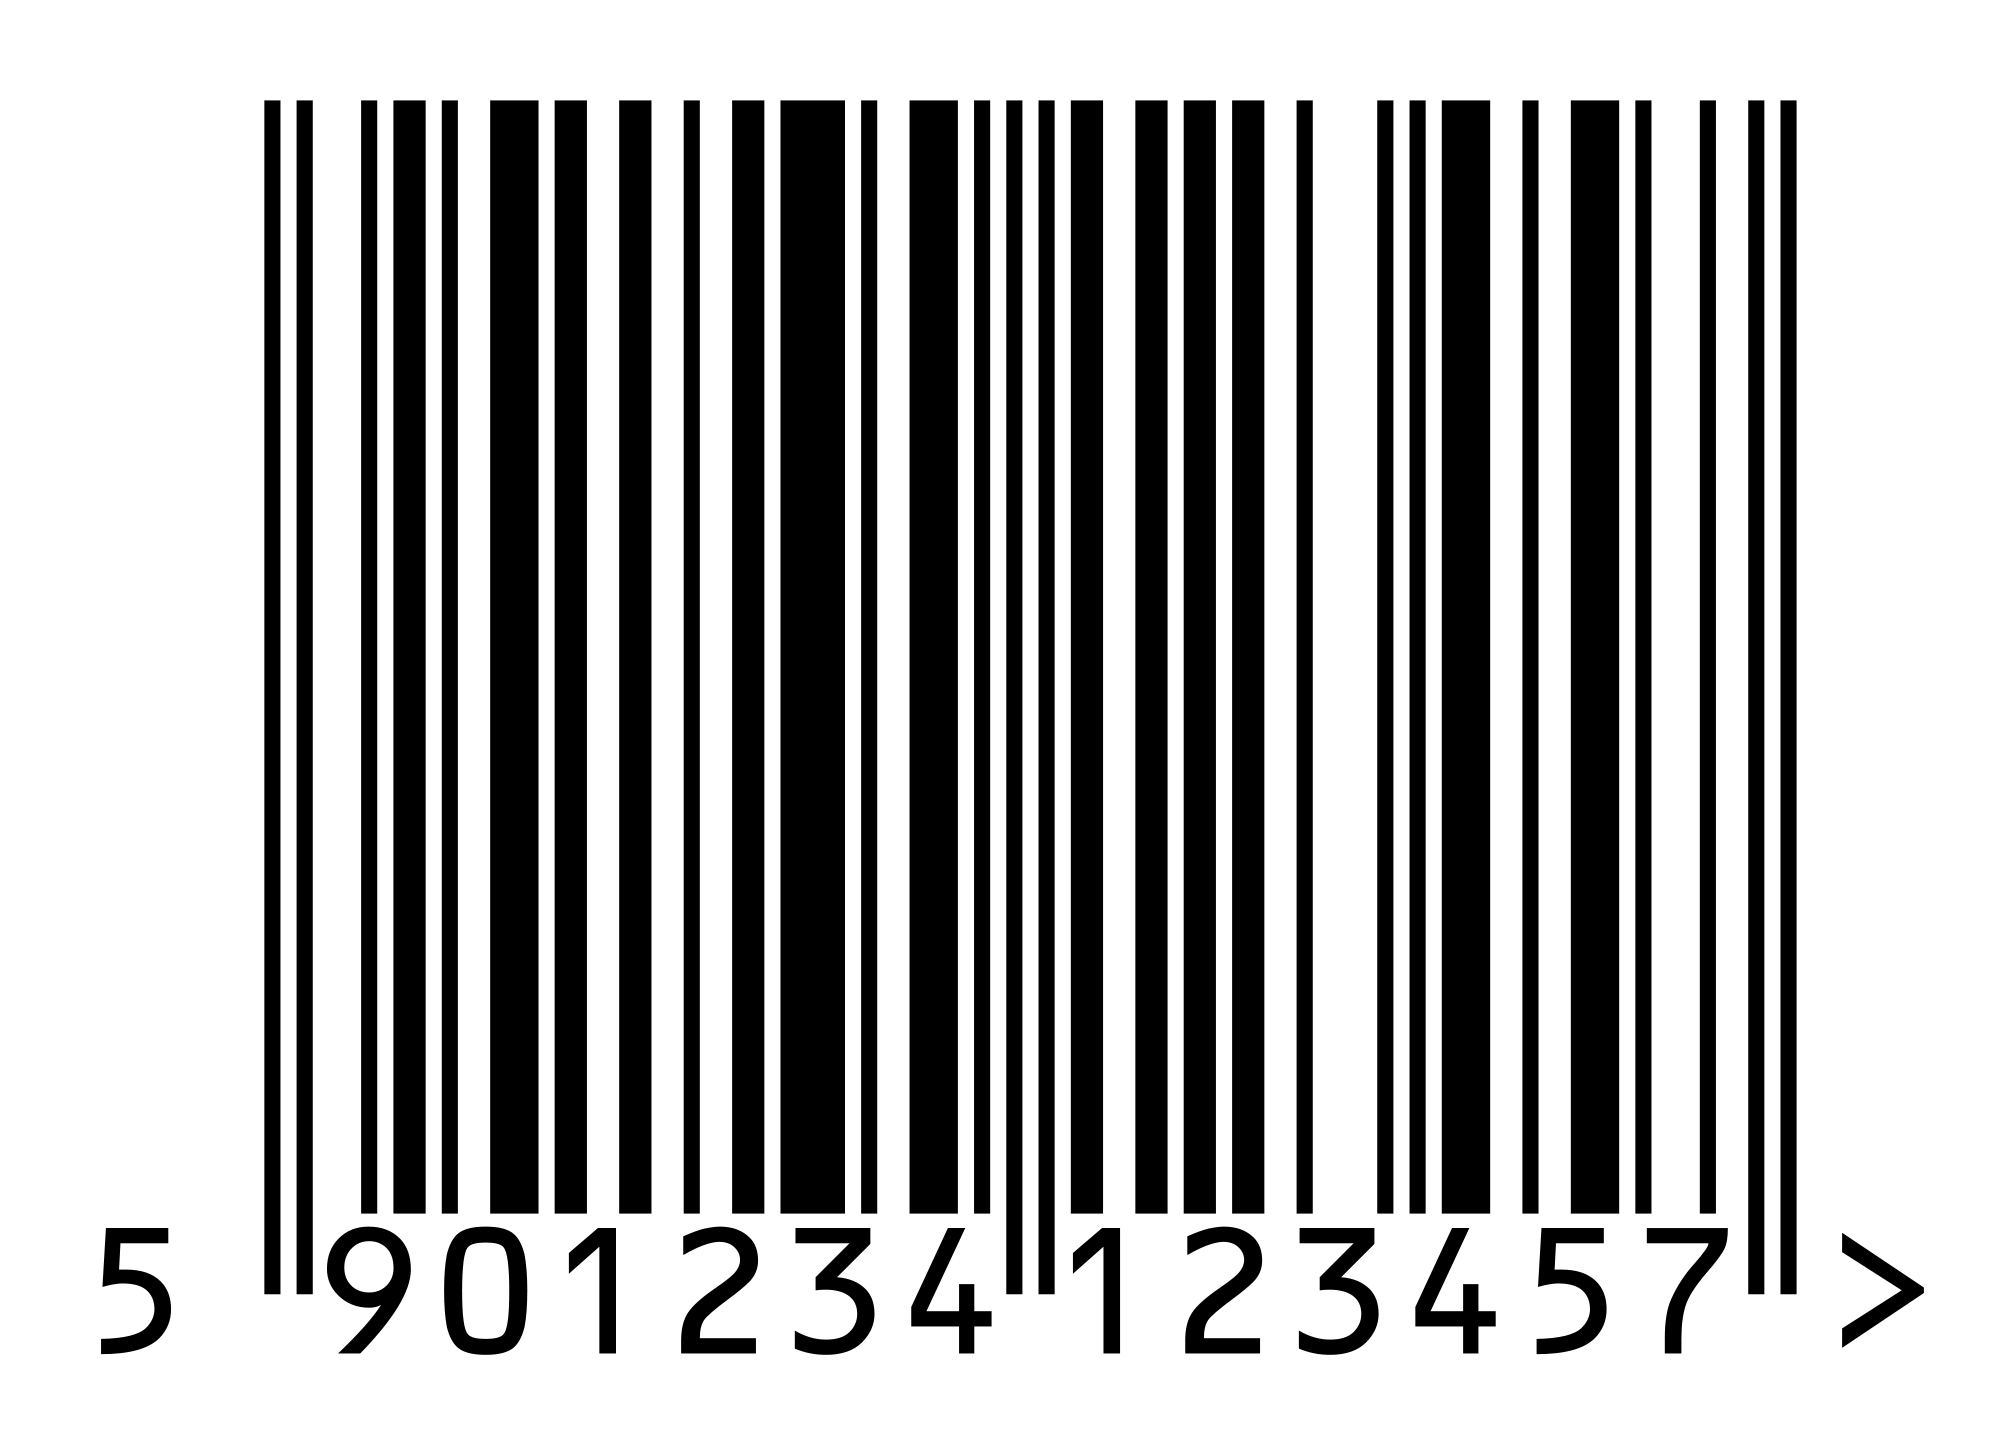
\includegraphics[width=0.25\textwidth]{Bilder/EAN_13.png}
	%\vspace{-0.2cm}
	\caption[EAN-13 Strichcode]{EAN-13 Strichcode\footnotemark}
	\label{barcode}
\end{figure}
\footnotetext{Quelle: \cite{Sakurambo2007}}
\pagebreak
\subsection{Zweidimensionale Barcodes}
Zweidimensionale Barcodes enthalten Informationen entlang ihrer X- und ihrer Y-Achse. Anders gesagt, horizontal werden andere Daten codiert als vertikal.
Damit der Code richtig entschlüsselt werden kann, muss ein Scanner beide Dimensionen simultan, das Symbol also als Ganzes erfassen. Dies ist möglich durch verschieben der Scanlinie eines Laserscanners oder durch verwenden eines Laserscannerarrays welches als Kamera fungiert. Ebenso ist der Einsatz einer Kamera möglich, die den Code anschließend durch bildverarbeitende Algorithmen entschlüsselt.

\subsubsection{Stapelcode}
Stapelcodes bestehen aus mehreren Lagen von linearen Barcodes, die vertikal übereinander angeordnet wurden.
Der spezielle Typ 'Composite Bar Code' besteht aus einem linearen und einem zweidimensionalen Part.

\subsubsection{Matrixcodes}
Matrixcodes codieren Daten durch benutzen von Zellen innerhalb einer Matrix (daher auch der Name). Diese benutzten Zellen werden für die Darstellung innerhalb des Symbols schwarz gefärbt. Jede Zelle innerhalb des Codes ist gleich groß. 
Vorteile der Matrixcodes: Es werden viele Daten auf kleinem Raum gespeichert, die Lesbarkeit ist hoch, der Code kann auch bei schlechter Druckqualität oder Beschädigung noch gelesen werden und unterstützt den vollen ASCII Zeichensatz.
Nachteil: Es benötigt eher eine Kamera als einen Laserscanner, um den Code zu lesen. 
\samepage
\paragraph{QR-Code}~

Der QR-Code (ausgeschrieben \textit{Quick-Response}) wurde 1994 von der japanischen Firma Denso entwickelt. Heute wird er hauptsächlich in der Automobilindustrie und als Smartphone-Code verwendet; hier vor allem für Mobile Ticketing beziehungsweise Mobile Marketing. Diese mobile Anwendung ist auch auf seine hohe Fehlertoleranz zurückzuführen. Da der QR-Code den Hauptteil dieser Arbeit ausmachen soll, finden sich weiter Informationen und Details im entsprechenden Kapitel.

\begin{figure}[htbp]%[7]{l}[0.5cm]{0.3\textwidth}
	\centering
%	\vspace{-0.65cm}
	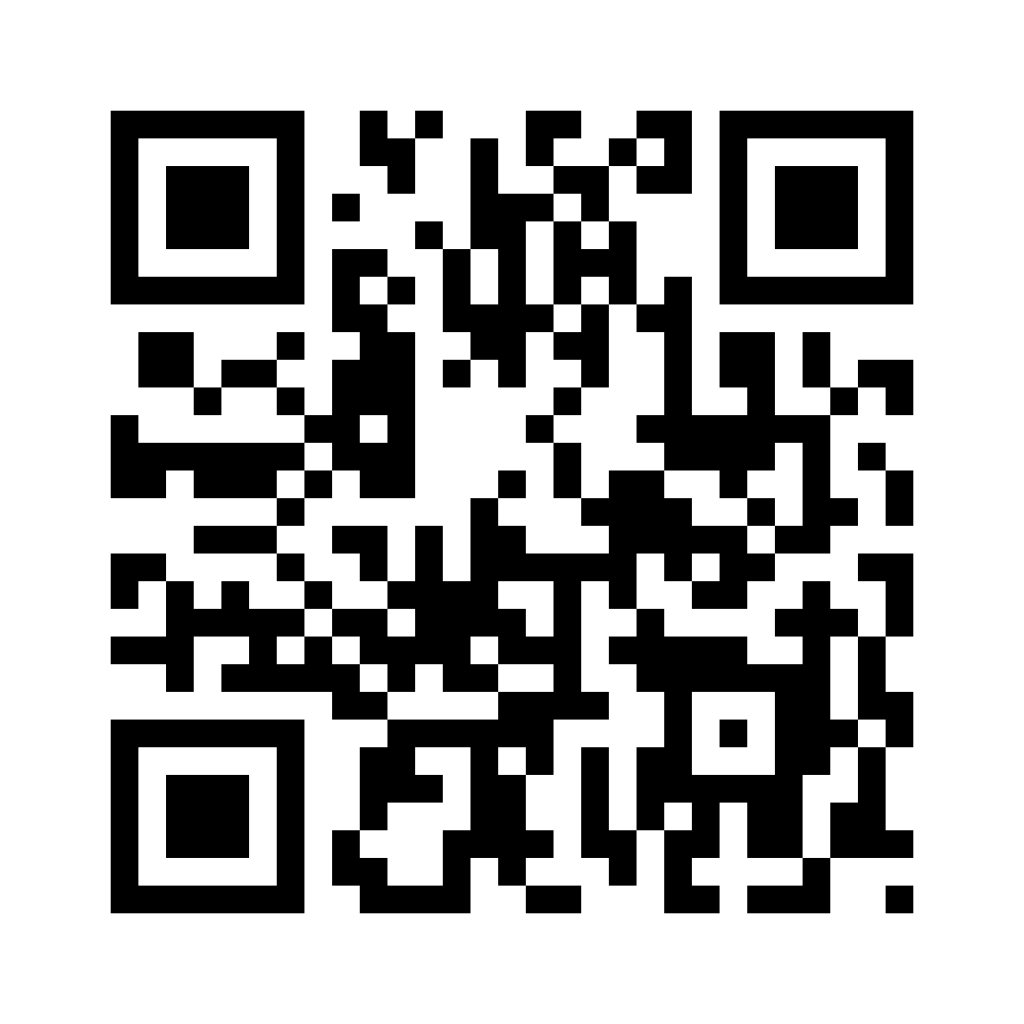
\includegraphics[width=0.25\textwidth]{Bilder/QR_Code.png}
%	\vspace{-0.2cm}
	\caption[QR-Code]{QR-Code\footnotemark}
	\label{fig:qrcode}	
\end{figure}~\\
\footnotetext{Quelle: \cite{brdall2009}}
\pagebreak
\paragraph{DataMatrix}~

Der DataMatrix-Code (siehe Abbildung~\ref{fig:datamatrix}) wurde gegen Ende der 1980er Jahre von der amerikanischen Firma Acuity Corp entwickelt. Da auch er eine hohe Fehlertoleranz aufweist, wird er heute vor allem zur Markierung kleiner Dinge verwendet, z.B. in der Produktion von Leiterplatten oder im Automobilbau. Die eingebaute Fehlerkorrektur verwendet den leistungsfähigen Reed-Solomon-Algorithmus\footnote{Der Reed-Solomon-Algorithmus ist ein in der Informationstechnik weit verbreiteter Algorithmus, um Fehler beim Übertragen von Daten zu korrigieren. Seine Funktionsweise ist nicht Bestandteil dieser Seminararbeit und kann in einschlägigen Quellen nachgelesen werden, beispielsweise unter \url{http://www-math.upb.de/~mathkit/Inhalte/MatheCD/i30.html}}. Innerhalb einer DataMatrix können bis zu 2335 Zeichen fixer Länge gespeichert werden.

\begin{figure}[htbp]%[6]{r}[0.9cm]{0.33\textwidth}
	\centering
%	\vspace{-0.65cm}
	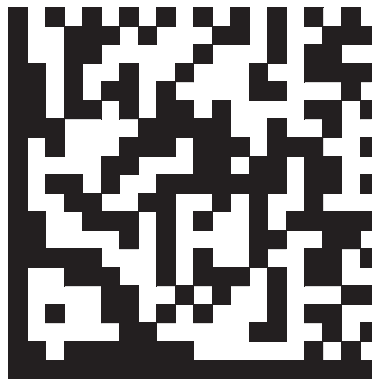
\includegraphics[width=0.23\textwidth]{Bilder/DataMatrix.png} 
%	\vspace{-0.2cm}
	\caption[DataMatrix]{DataMatrix\footnotemark}
	\label{fig:datamatrix}	
\end{figure}
\footnotetext{Quelle: \cite[23]{DatalogicScanning2007} }

\paragraph{Aztec-Code}~

Der Aztec-Code (siehe Abbildung~\ref{fig:aztec}) wurde im Jahr 1995 in der amerikanischen Firma Welch Allyn entwickelt.
Er ist normiert (ISO/IEC 24778) und wurde in Anlehnung an die Hochkultur der Azteken benannt, 
da die charakteristischen Quadrate in der Codemitte an eine aztekische Stufenpyramide aus der Vogelperspektive erinnern.\\ 

Auch der Aztec-Code ist sehr fehlertolerant (je nach Anwendungsfall können Daten auch bei einer Zerstörung von bis zu 40\% des Codes rekonstruiert werden). Er wird hauptsächlich in den Bereich Transport, Logistik und Verwaltung eingesetzt und dürften den meisten Lesern von den (mobilen) Fahrkarten der Deutschen Bahn bekannt sein, da der Internationale Eisenbahnverband \textit{UIC} den Aztec-Code als Standard für Fahrkarten definiert hat.\\

\begin{figure}[htbp]%[8]{r}[0.9cm]{0.35\textwidth}
	\centering
%	\vspace{-0.35cm}
	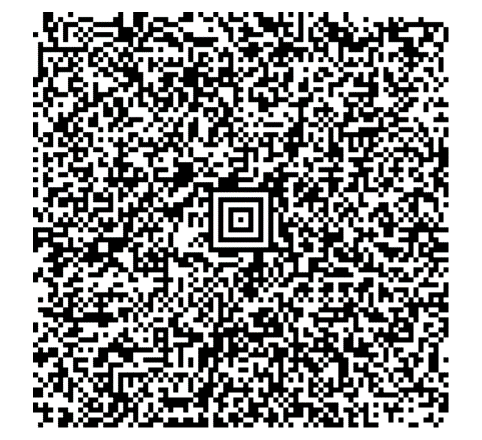
\includegraphics[width=0.3\textwidth]{Bilder/Aztec_Code.png} 
	%\vspace{-0.2cm}
	\caption[Aztec-Code]{Aztec-Code, wie er bei der Deutschen Bahn in der DB-Navigator-App als Handy-Ticket verwendet wird\footnotemark}
	\label{fig:aztec}	
\end{figure}
\footnotetext{Quelle: Christian Wernet, Handy-Ticket für eine Fahrt von Haslach i.K. nach Bühl(Baden) am 18.11.2016}

\paragraph{MaxiCode}~

Der MaxiCode ist eine besondere Form der Matrixcodes. Im Gegensatz zu den anderen Matrix besitzt er eine festgelegte Größe von 25,4 x 25,4 mm und besteht nicht aus quadratischen, sondern aus hexagonalen Modulen. Er wurde 1989 bei der amerikanischen Firma \textit{United Parcel Service (UPS)} entwickelt und wird zur Sortierung und Verfolgung von Paketen benutzt. Dabei ist von Vorteil, dass er omnidirektional gelesen werden kann und einen vergleichsweise begrenzten Informationsgehalt besitzt; eine primäre und eine sekundäre Information. Die primäre Nachricht enthält üblicherweise die Postleitzahl, die sekundäre die genaue Zieladresse. Generell gesprochen, können mit dem MaxiCode 93 ASCII-Zeichen oder 138 numerische Zeichen fester Länge codiert werde.
Da auch der MaxiCode den Reed-Solomon-Algorithmus zur Rekonstruktion verwendet, können selbst bei einer Zerstörung von bis zu 25\% des Codes noch alle Informationen rekonstruiert werden. \cite{DatalogicScanning2007} \cite{Lipinski2016} 
\pagebreak
\begin{figure}[htbp]%[1]{r}[0cm]{\textwidth}
	\centering
%	\vspace{-0.35cm}
	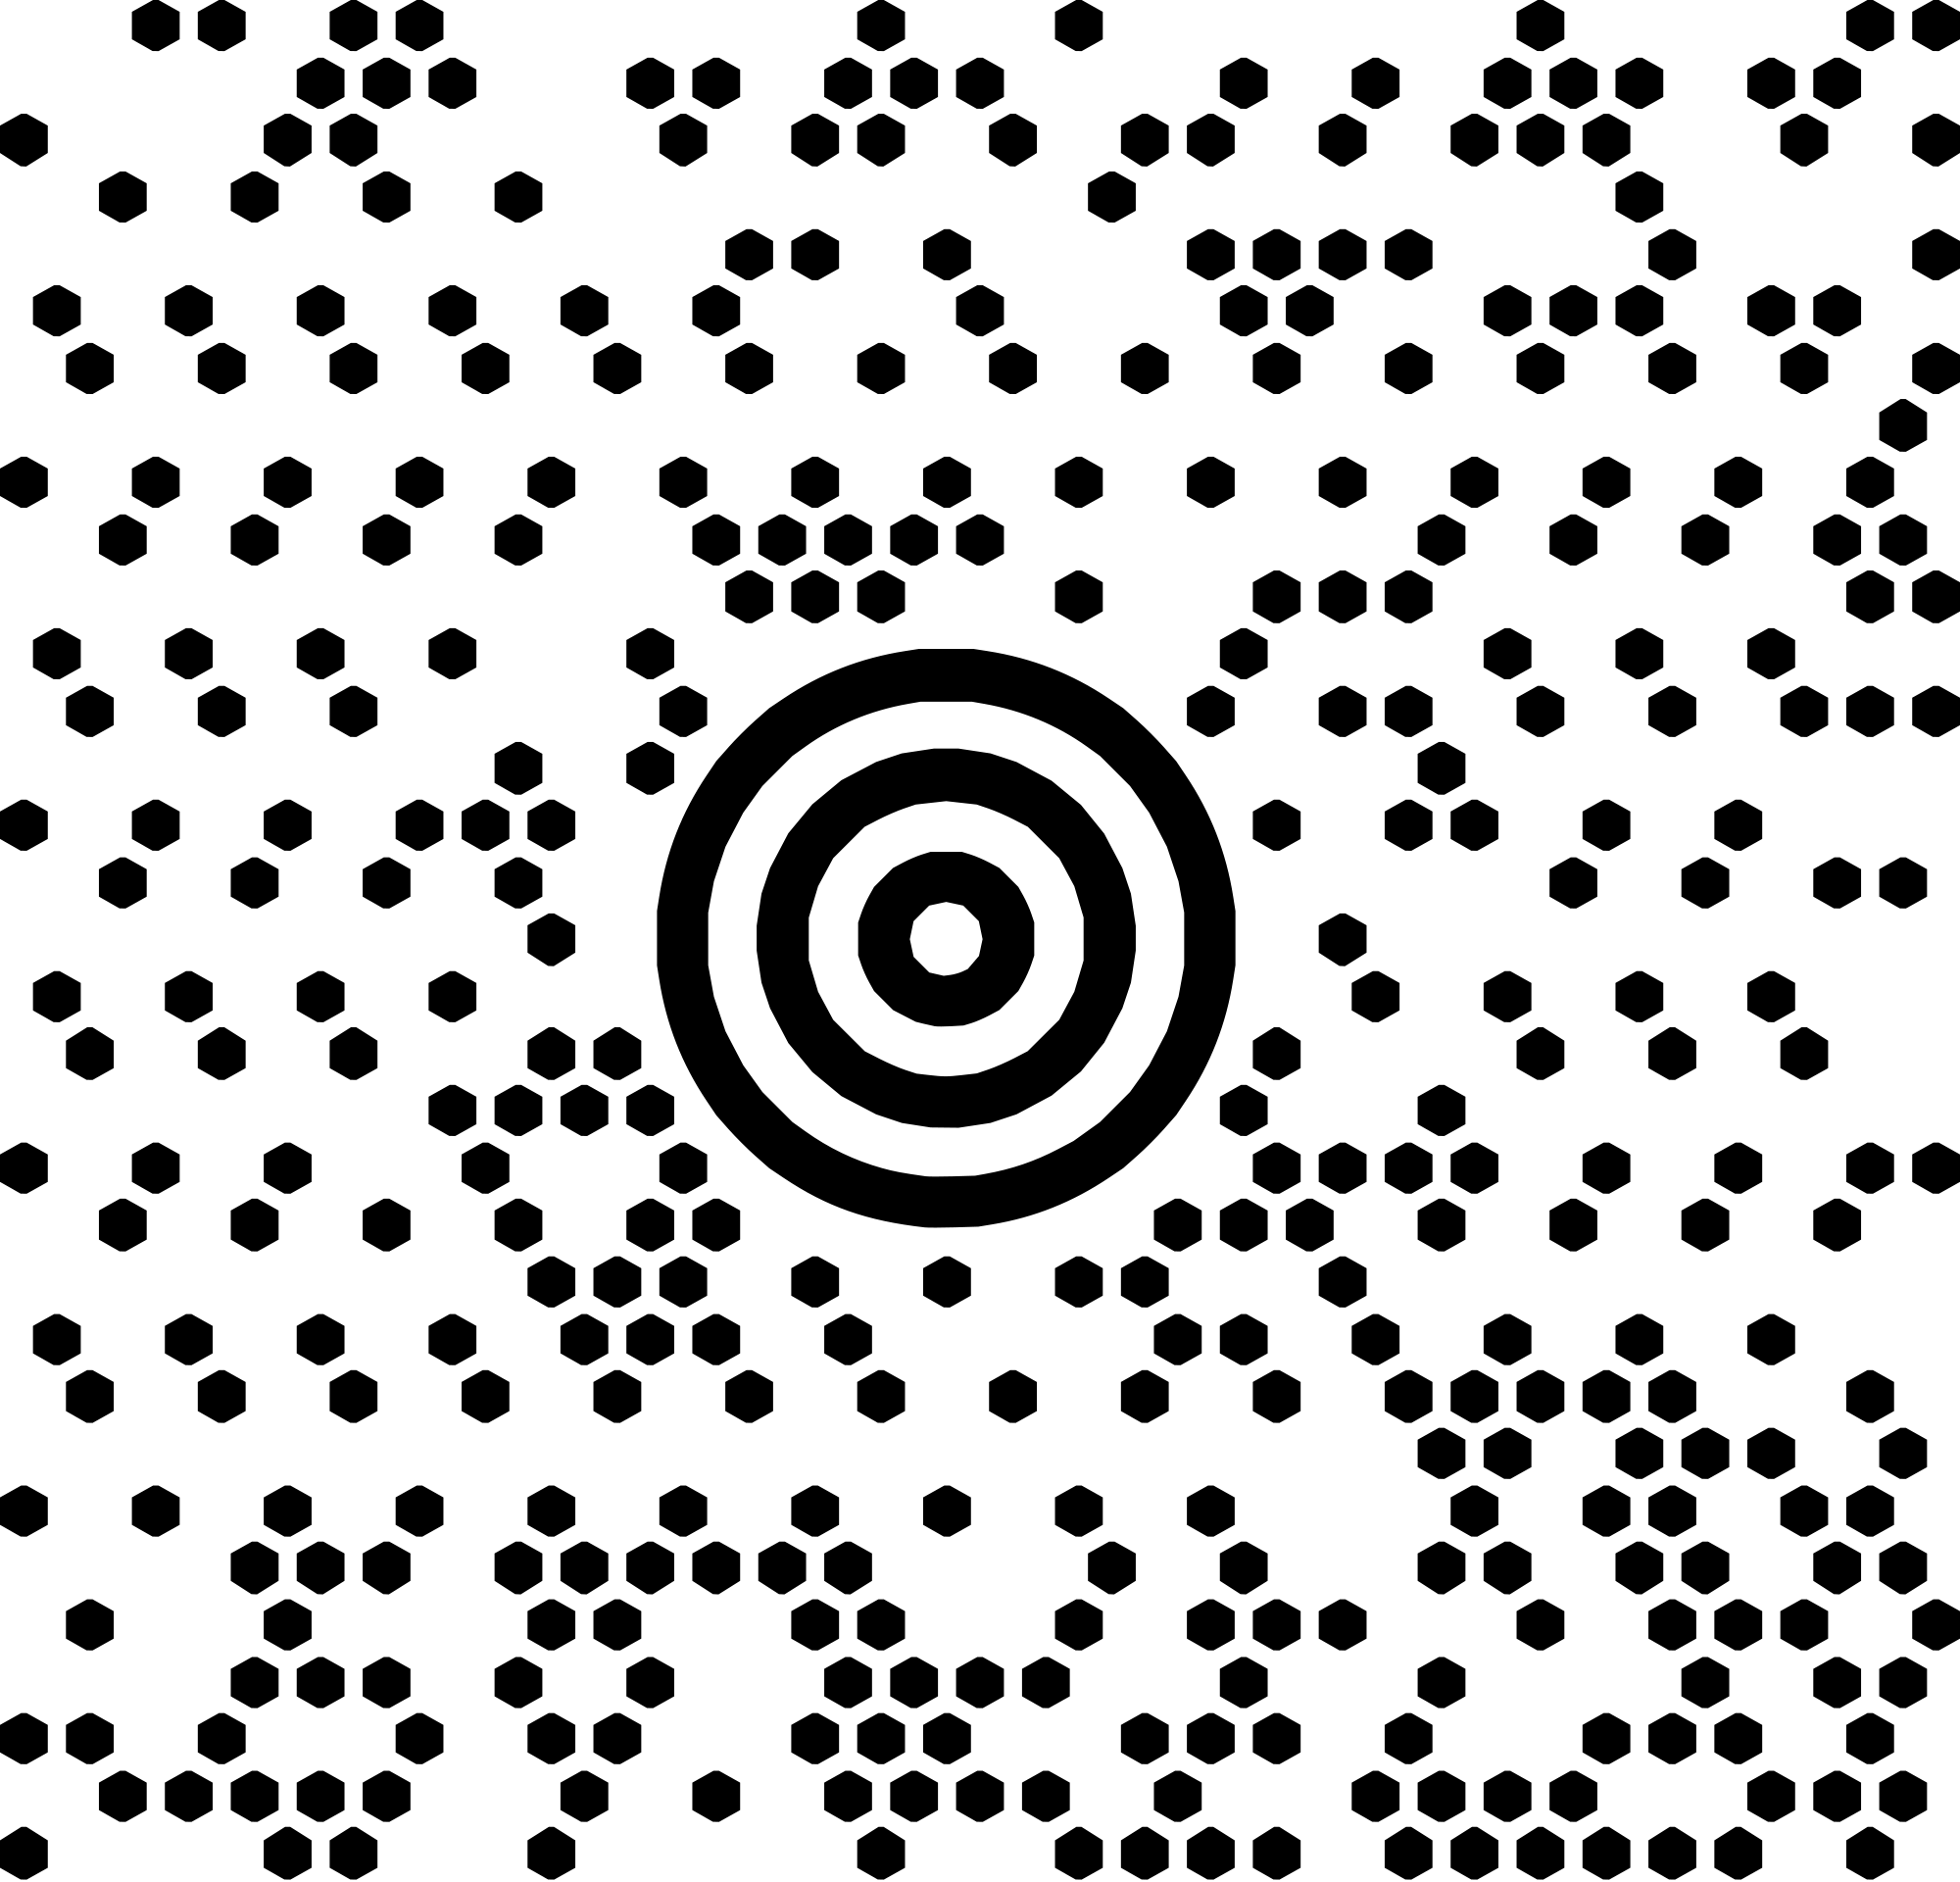
\includegraphics[width=0.25\textwidth]{Bilder/MaxiCode.png} 
	%	\vspace{0.2cm}
	\caption[MaxiCode]{MaxiCode, der den Inhalt "Wikipedia, the free encyclopedia" codiert.\footnotemark}
	\label{fig:maxicode}	
\end{figure}
\footnotetext{Quelle: \cite{Darco2008}}

\subsection{Dreidimensionale und vierdimensionale Barcodes}
Es gibt zwei verschiedene Arten von Barcodes, die als 3D-Code bezeichnet werden:
Zum einen die fühlbaren Codes mit unterschiedlichen Erhebungen und zum anderen die Farbcodes oder auch "farbige QR-Codes", bei denen die Farbe die dritte Dimension darstellt.
Das amerikanische Unternehmen Microsoft hat im Jahr 2007 den sogenannten "High Capacity Color Barcode (HCCB)" vorgestellt. Mit diesem wurde die Informationsdichte des Barcodes durch "benutzen verschiedener Barcode-Symbolformen in Kombination mit verschiedenen Farben pro Symbol"\cite{Paradiso2007}.
In Googles Play Store wird passend zu diesen Code eine Reader-Application namens "\href{https://play.google.com/store/apps/details?id=com.microsoft.tag.app.reader}{Microsoft Tag, QR \& NFC Reader} " von Microsoft Tag angeboten.
\begin{figure}[htbp]%[8]{r}[0.9cm]{0.35\textwidth}
	\centering
	%	\vspace{-0.35cm}
	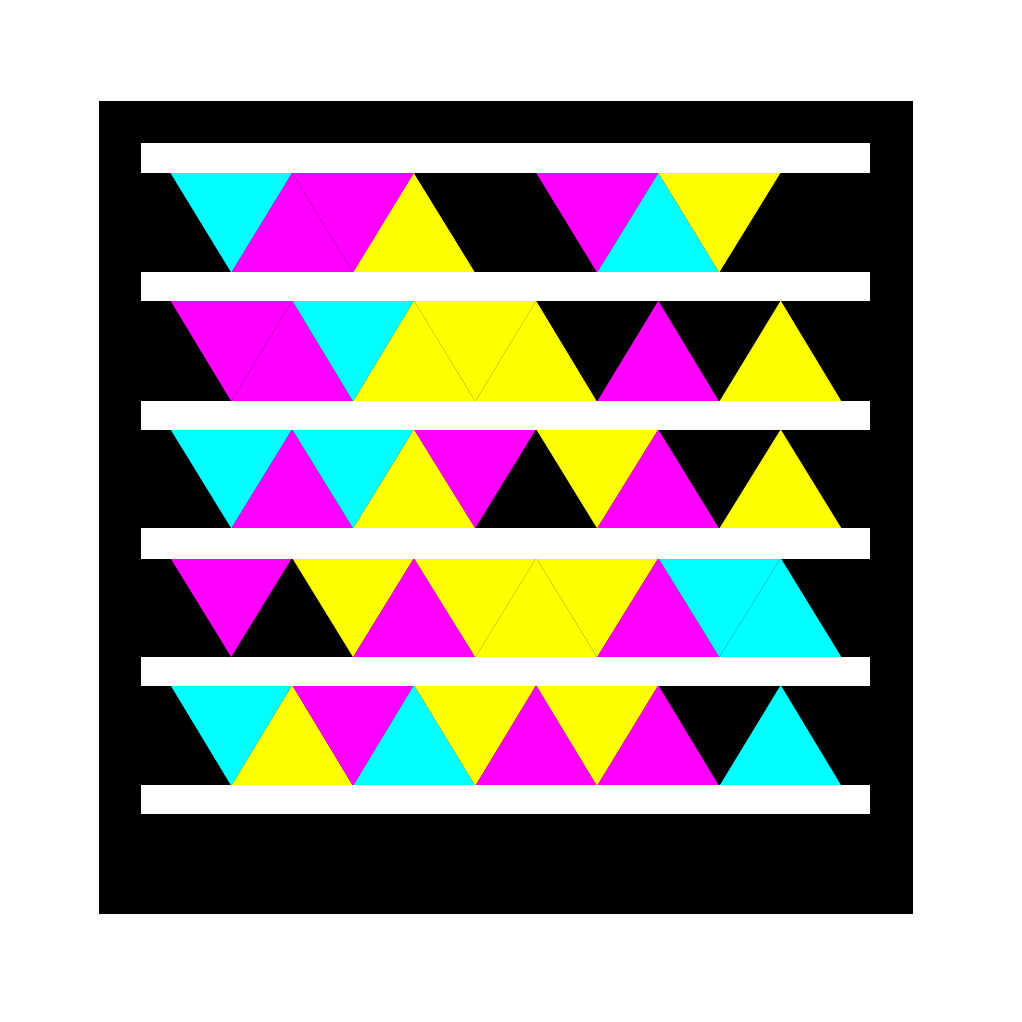
\includegraphics[width=0.3\textwidth]{Bilder/HCCB.png} 
	\vspace{-0.2cm}
	\caption[High Capacity Color Barcode]{High Capacity Color Barcode, der die URL \url{https://en.wikipedia.org/wiki/High_Capacity_Color_Barcode} codiert.\footnotemark}
	\label{fig:hccb}	
\end{figure}
\footnotetext{Leider ist der Code nicht mehr aktiv (Stand 08.12.2016). Quelle: \cite{zayani2009}}~\\
Der Nachteil dieser Farbcodes ist jedoch, dass Farbe mit der Zeit verblasst oder abblättert, sodass entsprechende Codes über kurz oder lang unlesbar werden würden.\\
Ein "{}echter"{} 3D-Code würde jedoch nicht einfach nur Farbinformationen zu einem bestehenden 2D-Code hinzufügen, sondern Informationen auch in der z-Achse codieren. 

Hierbei wäre die Informationsdichte auch wesentlich höher als bei einfachen farbangereicherten 2D-Codes.  Umgangssprachlich würde man in diesem Fall von einem Hologramm sprechen. Da jedoch die aktuelle Technik noch nicht weit genug ist, spielt diese Art von 3D-Codes noch keine Rolle in der klassischen Datenerfassung. \cite{EtiscanGmbH2016}\\
Auch vorstellbar wäre das Einbeziehen der vierten Dimension; der Zeit. 2007 entwickelten Forscher an der Bauhaus Universität in Weimar einen 4D-Code. Dieser bestand aus Bewegtbildern oder auch Animationen, die eingescannt werden können. Ein Anwendungsgebiet wäre mit diesem Code zum Beispiel die Datenübertragung zwischen zwei Smartphones \cite{Unglaube2015}.

~\pagebreak
